\section{Plots of Estimated Legislators' Ideological Positions\label{sec:Plots full}}

This section plots estimated legislators' ideological positions. \autoref{fig:session-plot} plots for the ideological positions of two major parties at a frequency of session. From session 7-1 (the electoral reform in 2008), legislators from the two-major parties underwent a phase of drastic ideological diverging, as the distributions for both parties started moving to both pole (political polarisation).  \autoref{fig:term-plot} displays estimated legislators' ideological positions for all minor parties (DPP and KMT excluded) at a frequency of year. \autoref{fig:individual_point} plots individual legislator's ideal point from two major parties, grouped by year.

\begin{figure}[H]
\caption{Estimated Legislators' Positions for Two Major Parties across the Legislative Sessions \label{fig:session-plot} }
\centering{}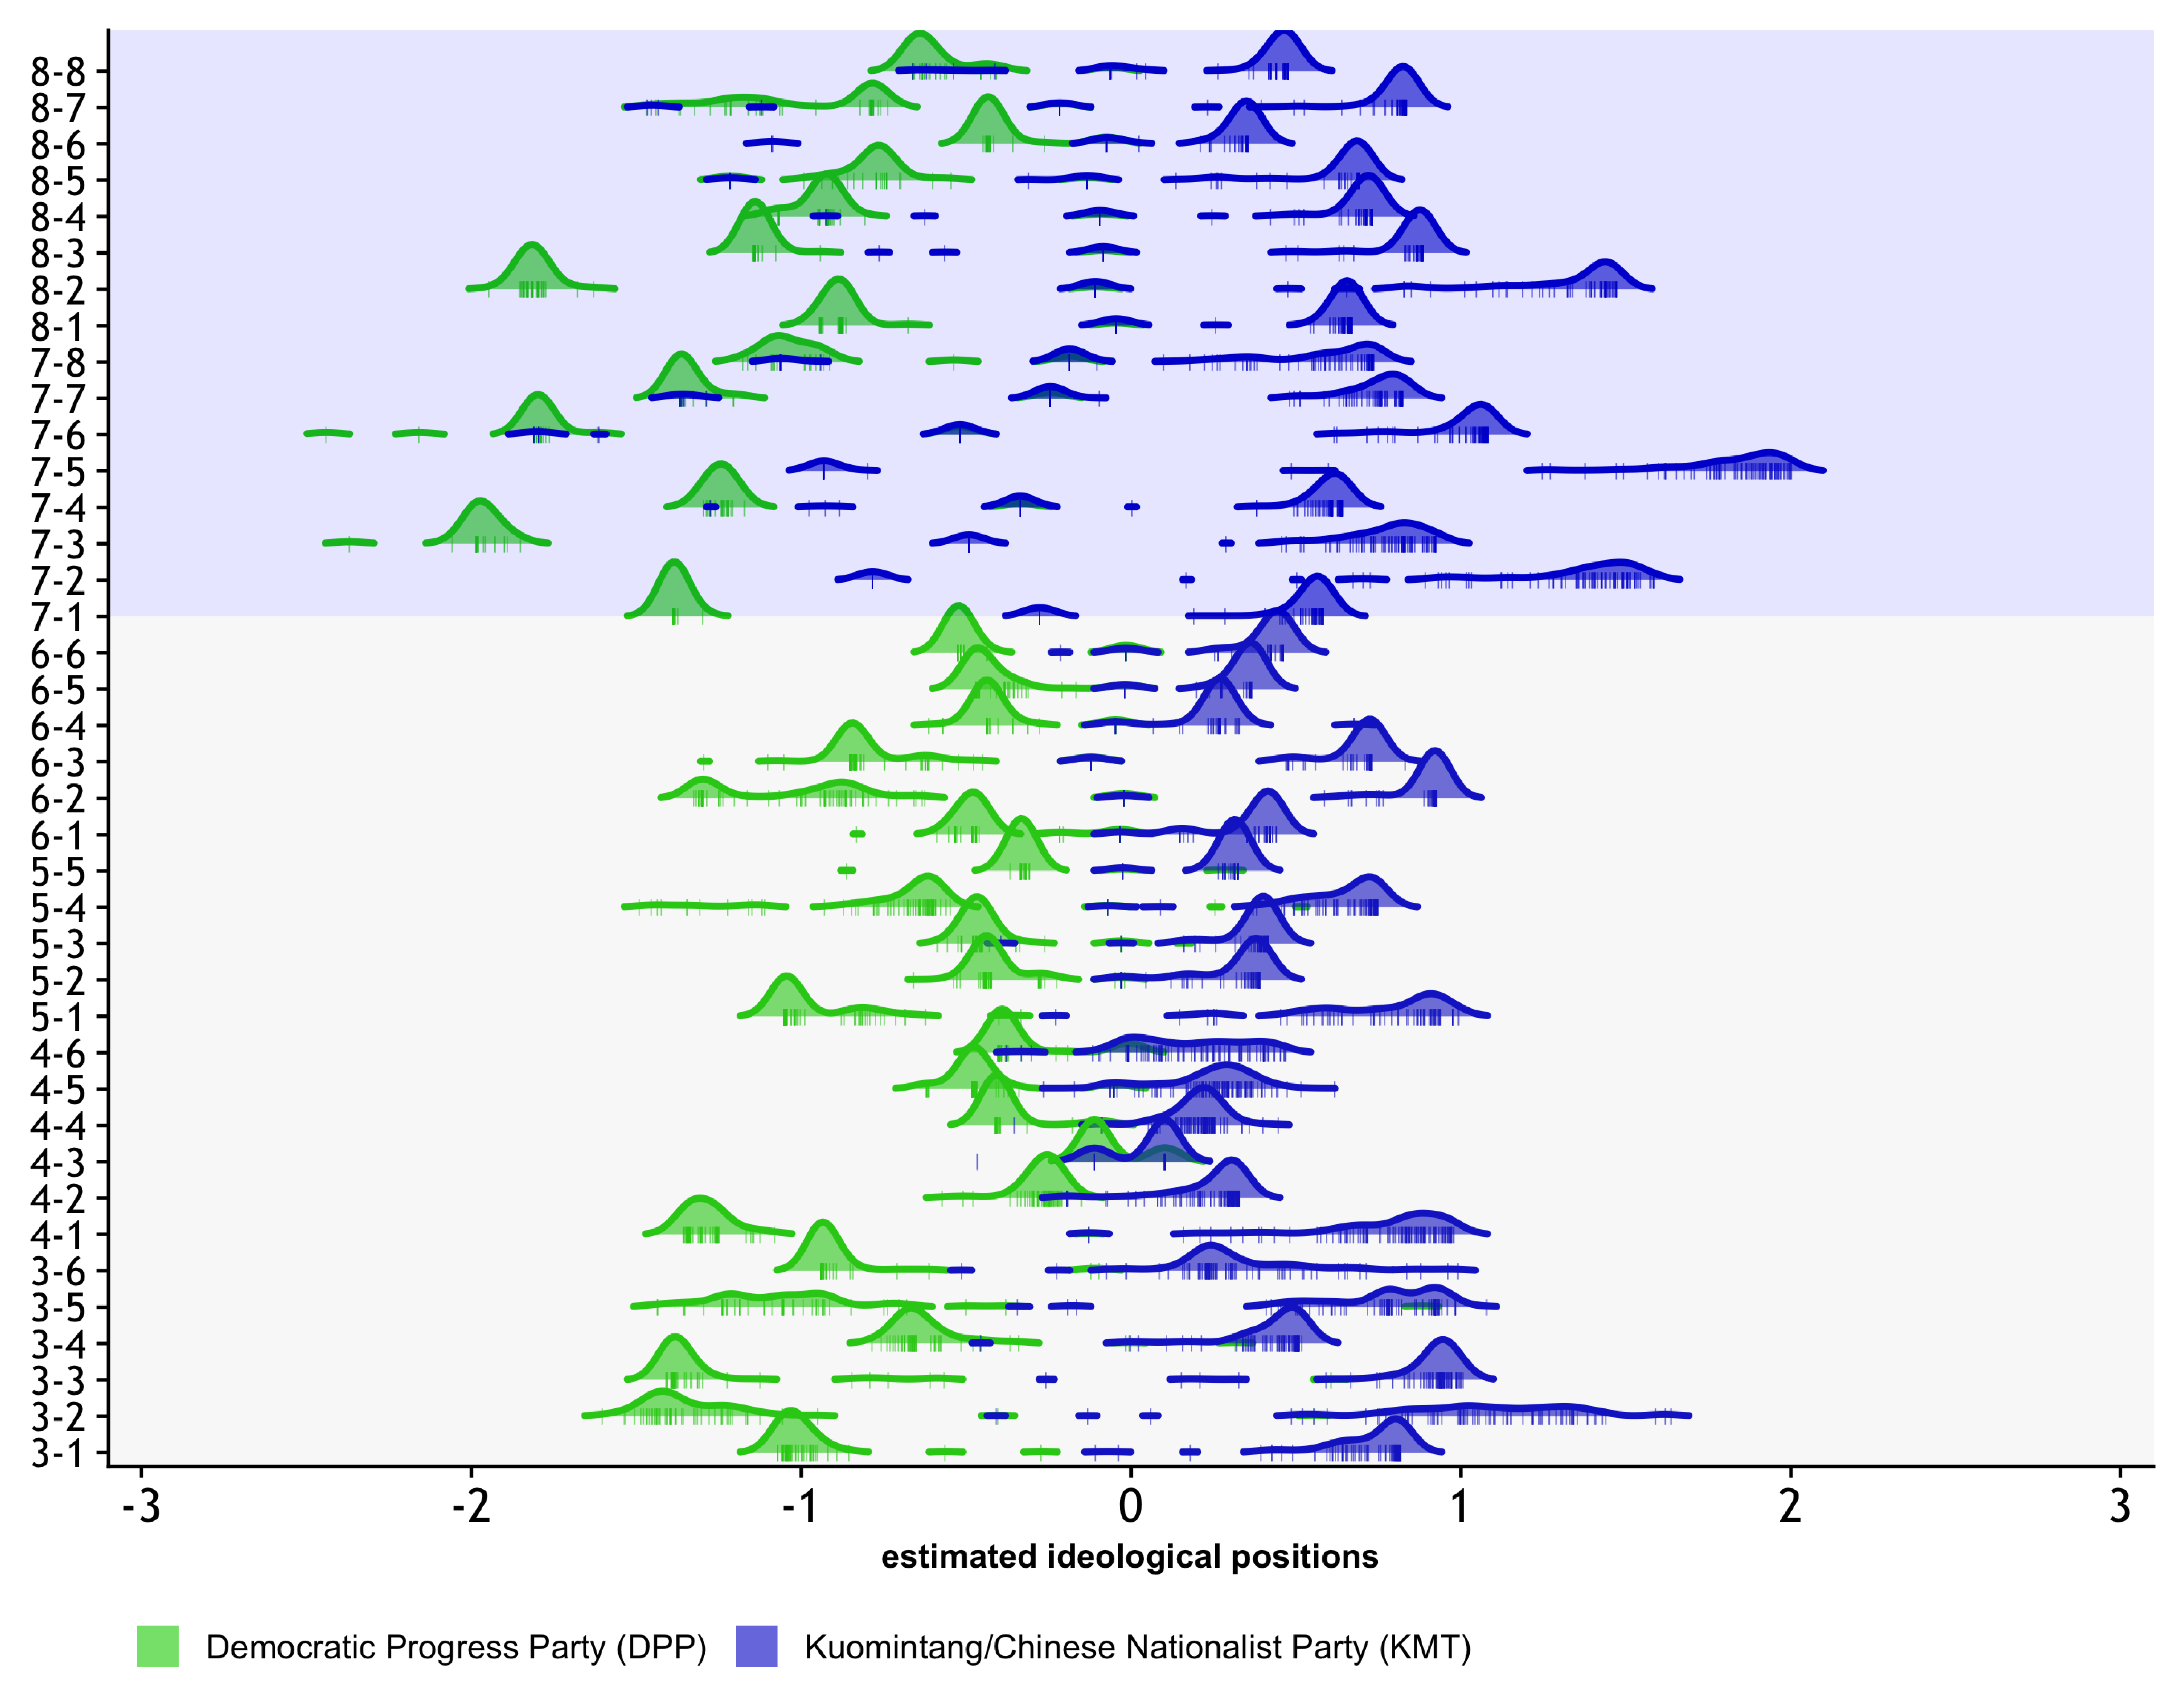
\includegraphics[scale=0.15]{02-Chapter-Two/image/major_postions_session}
\end{figure}

\begin{figure}[H]
\caption{Estimated Legislators' Ideological Positions for Small Parties across Years\label{fig:term-plot}}
\centering{}\includegraphics[scale=0.15]{02-Chapter-Two/image/minor_postions_year}
\end{figure}

\begin{figure}[H]
\caption{Individual Legislator' Ideal Point on a Single Dimension
for Two Major parties \label{fig:individual_point}}\centering{}\includegraphics[scale=0.14]{02-Chapter-Two/image/individual_point}
\end{figure}

\clearpage

\section{\centering Robustness Estimation using Sub-samples\label{sec:robustness-check}}
\subsection{Inter-party Competition and Distances\label{subsec:robustness-inter-party}}

I replicate the estimations results from Section \ref{subsec:disunity-in-co-partisan} using data of DPP and KMT separately to ensure the result of between-party polarisation is not solely driven by any big parties. \autoref{tab:Inter_DM} reports the outcomes. Column 1 and 2 display the result using DPP and KMT respectively. The variable of \textbf{electoral reform } is statistically significant positive (at 1\% critical level in both columns), implying that the electoral reform significantly increases between-party ideological distance (political polarisation) regardless of the party-affiliation, consistent with the results found in \autoref{tab:intra-estimation}.


\begin{table}[H]
\caption{Legislator-level Interparty Distance\label{tab:Inter_DM}}
\centering{}%
\begin{tabular}{lcc}
    \toprule 
    \multicolumn{3}{l}{\textbf{Dependent variable:}}                          \tabularnewline
    \multicolumn{3}{l}{Interparty Legislator Ideological Distance}           \tabularnewline
    \midrule
                                & \textbf{DPP} & \textbf{KMT}                 \tabularnewline
    \midrule
electoral reform                & 23.000$^{***}$ & 13.132$^{***}$             \tabularnewline
                                & (2.916)        & (0.859)                    \tabularnewline
year                            & -0.205$^{***}$ & -0.263$^{***}$             \tabularnewline
                                & (0.015)        & (0.012)                    \tabularnewline
year $\times$ electoral reform  & -1.045$^{***}$ &  -0.460$^{***}$            \tabularnewline
                                & (0.153) & (0.047)                           \tabularnewline
marginal winning shares         & 0.017       & 0.250                         \tabularnewline
                                & (0.281)       & (0.136)                     \tabularnewline
intercept                       & 3.222$^{***}$ & 3.268$^{***}$               \tabularnewline
                                & (0.395)       & (0.316)                     \tabularnewline
legislator attributes           &     $\checkmark$    & $\checkmark$          \tabularnewline
district fixed effects          &     $\checkmark$    & $\checkmark$          \tabularnewline
    \midrule
No. of observations             & 1623          & 2547                        \tabularnewline
Adjusted R$^{2}$                & 0.28          & 0.27                        \tabularnewline
Prob > F                        & 0.00          & 0.00                        \tabularnewline
    \midrule
\multicolumn{3}{l}{{\footnotesize{}Robust standard errors are reported in parentheses. Asterisk}}   
                                                                              \tabularnewline
\multicolumn{3}{l}{{\footnotesize{}indicates significant level: {*}: p < 0.10; {*}{*}:p < 0.05; {*}{*}{*}:p < 0.01.}}                                                                                               \tabularnewline
\end{tabular}
\end{table}

\subsection{Disunited Distances between Co-partisan Legislators \label{subsec:disunity-robust}}

This section replicates the estimations results from Section \autoref{subsec:disunity-in-co-partisan} using observations of DPP and KMT separately to ensure the result of within-party disunity is not solely driven by any big parties. \autoref{tab:Intra_DM} reports the outcomes. Column 1 and 2 display the result using DPP and KMT respectively. The variable of \textbf{electoral reform} is statistically significant positive (at 5\% and 1\% critical level in column 1 and 2, respectively), implying that the electoral reform significantly increased within-party ideological distance regardless of the party-affiliation, consistent with the results found in  \ref{tab:intra-estimation}.

\begin{table}[H]
\caption{Legislator-level Intraparty Distance\label{tab:Intra_DM}}
\centering{}%
\begin{tabular}{lcc}
\toprule 
\multicolumn{3}{l}{\textbf{Dependent variable:}}                      \tabularnewline
\multicolumn{3}{l}{Intraparty Ideological Distance}     \tabularnewline
\midrule
                             & \textbf{DPP}  & \textbf{KMT}           \tabularnewline
\midrule
electoral reform             & 0.816$^{**}$  & 2.675$^{***}$          \tabularnewline
                             & (0.323)       & (0.411)                \tabularnewline
year                         & -0.007$^{**}$ & -0.005$^{**}$          \tabularnewline
                             & (0.003)       & (0.002)                \tabularnewline
year $\times$ electoral reform  & -0.037$^{**}$     & -0.123$^{***}$  \tabularnewline
                                & (0.017)           & (0.021)         \tabularnewline
marginal winning shares         & 0.046             & 0.018           \tabularnewline
                                & (0.069)           & (0.136)         \tabularnewline
intercept                       & 0.066             & -0.081          \tabularnewline
                                & (0.070)           & (0.124)         \tabularnewline
legislator attributes           & $\checkmark$      & $\checkmark$    \tabularnewline
district fixed effects          & $\checkmark$      & $\checkmark$    \tabularnewline
\midrule
No. of observations             & 1623              & 2547            \tabularnewline
Adjusted R$^{2}$                & 0.03              & 0.05            \tabularnewline
Prob > F                        & 0.01              & 0.00            \tabularnewline
\midrule

\multicolumn{3}{l}{\footnotesize{}Robust standard errors are reported in parentheses. Asterisk }           \tabularnewline
\multicolumn{3}{l}{\footnotesize{}indicates significant level: {*}: p < 0.10; {*}{*}: p < 0.05; {*}{*}{*}:}\tabularnewline
\multicolumn{3}{l}{\footnotesize{}p < 0.01.}                                                               \tabularnewline
\end{tabular}
\end{table}

\clearpage

\section{Addressing the Heterogeneity in Bills Voted across Year\label{sec:Addressing-the-heterogeneity}} 

Then, there is also the heterogeneity in years that could impact the legislature ideological position through voting decision, due to multiple reasons. First, in some years, bills voted were more likely to cause inter- or intraparty disagreement and thus, dispersion in ideological points. Second, in some years, the major social activities or events happened that also could cause disagreement or conflicts in the legislature. For example, in 2006, there was a mass campaign (\textit{Million Voices against Corruption}, President Chen Must Go) led by former DPP Chairman Shih Ming-teh (施明德) to pressure the President Chen Shui-bian (陳水扁) to resign. Therefore, I address the problem concerning the heterogeneity in year by controlling for as many years as possible.\footnote{Some years (2007, 2014 and 2015) are omitted due to multi-collinearity.}  \autoref{tab:heterogeneity of bills} reports the estimation results for inter-party analysis, with (column 2) or without controlling for other effects (column 1). As you can see, \textbf{electoral reform }is still statistically significant positive (at 1\% critical level) and are robust, meaning that the electoral reform caused higher level of inter-party dispersion between KMT and DPP, even if I introduce additional year dummies and control for the passage of time and other attributes.\footnote{Almost all year dummies are statistically significant at the 1\% critical level for both regressions, except year 2008. Estimated coefficients and standard errors for year dummies are omitted due to space limit.}  \autoref{tab:heterogeneity of bills} reports the estimation results for intraparty analysis, with (column 2) or without controlling for other effects (column 1). Similar results are obtained.

\begin{table}[ht]
\caption{Interparty Distance by Controlling for the Heterogeneity Effects from Different Years \label{tab:heterogeneity of bills}}
\centering{}%
\begin{tabular}{lcc}
\toprule 
\multicolumn{3}{l}{\textbf{Dependent variable:}}                                                            \tabularnewline
\multicolumn{3}{l}{Inter-party Ideological Distance}                                                        \tabularnewline
\midrule
                                & \footnotesize{\textbf{Interaction}} &                                      \tabularnewline
                                & \footnotesize{\textbf{+ Years}}     & \footnotesize{\textbf{(+ Controls)}} \tabularnewline
\midrule
\footnotesize{electoral reform} & \footnotesize{6.18$^{***}$}  & \footnotesize{6.401$^{***}$}  \tabularnewline
                                & \footnotesize{(0.818)}       & \footnotesize{(0.968)}        \tabularnewline
\footnotesize{year}             & \footnotesize{-0.361$^{***}$}& \footnotesize{-0.355$^{***}$} \tabularnewline
                                & \footnotesize{(0.010)}       & \footnotesize{(0.012)}        \tabularnewline
\footnotesize{year$\times$ electoral reform}   & \footnotesize{-0.147$^{***}$}   & \footnotesize{-0.158$^{***}$} \tabularnewline
                                & \footnotesize{(0.042)}       & \footnotesize{(0.050)}       \tabularnewline
\footnotesize{intercept}        & \footnotesize{5.050$^{***}$} & \footnotesize{5.598$^{***}$} \tabularnewline
                                & \footnotesize{(0.120)}       & \footnotesize{(0.246)}       \tabularnewline
\footnotesize{1997}             & $\checkmark$         & $\checkmark$  \tabularnewline
\footnotesize{1998}             & $\checkmark$         & $\checkmark$  \tabularnewline
\footnotesize{1999}             & $\checkmark$         & $\checkmark$  \tabularnewline
\footnotesize{2000}             & $\checkmark$         & $\checkmark$  \tabularnewline
\footnotesize{2001}             & $\checkmark$         & $\checkmark$  \tabularnewline
\footnotesize{2002}             & $\checkmark$         & $\checkmark$  \tabularnewline
\footnotesize{2003}             & $\checkmark$         & $\checkmark$  \tabularnewline
\footnotesize{2004}             & $\checkmark$         & $\checkmark$  \tabularnewline
\footnotesize{2005}             & $\checkmark$         & $\checkmark$  \tabularnewline
\footnotesize{2006}             & $\checkmark$         & $\checkmark$  \tabularnewline
\footnotesize{2005}             & $\checkmark$         & $\checkmark$  \tabularnewline
\footnotesize{2009}             & $\checkmark$         & $\checkmark$  \tabularnewline
\footnotesize{2010}             & $\checkmark$         & $\checkmark$  \tabularnewline
\footnotesize{2011}             & $\checkmark$         & $\checkmark$  \tabularnewline
\footnotesize{2012}             & $\checkmark$         & $\checkmark$  \tabularnewline
\footnotesize{2013}             & $\checkmark$         & $\checkmark$  \tabularnewline
\footnotesize{legislator attributes}       &           & $\checkmark$  \tabularnewline
\footnotesize{party dummies}               &           & $\checkmark$  \tabularnewline
\footnotesize{district fixed effects}      &           & $\checkmark$  \tabularnewline
\midrule
\footnotesize{No. of Observations}         & \footnotesize{5663}      & \footnotesize{4170}         \tabularnewline
\footnotesize{Adjusted R$^{2}$}            & \footnotesize{0.53}      & \footnotesize{0.51}         \tabularnewline
\footnotesize{Prob > F}                    & \footnotesize{0.00}      & \footnotesize{0.00}         \tabularnewline
\midrule
\multicolumn{3}{l}{{\footnotesize{}Robust standard errors are reported in parentheses.}}           \tabularnewline
\multicolumn{3}{l}{{\footnotesize{}Asterisk indicates significant level: {*}: p < 0.10; {*}{*}:}}    \tabularnewline
\multicolumn{3}{l}{{\footnotesize{} p < 0.05; {*}{*}{*}:p < 0.01.}}                                   \tabularnewline
\end{tabular}
\end{table}

\begin{table}[ht]
\caption{Intraparty Distance by Controlling for the Heterogeneity Effects from Different Years \label{tab:heterogeneity of bills-1}}
\centering{}%
\begin{tabular}{lcc}
\toprule 
\multicolumn{3}{l}{\textbf{Dependent variable:}}                                                            \tabularnewline
\multicolumn{3}{l}{\footnotesize{Inter-party Ideological Distance}}                                                        \tabularnewline
\midrule
                                & \footnotesize{\textbf{Interaction}} &                                      \tabularnewline
                                & \footnotesize{\textbf{+ Years}}     & \footnotesize{\textbf{(+ Controls)}} \tabularnewline
\midrule
\footnotesize{electoral reform} & \footnotesize{1.696$*$}       & \footnotesize{1.747$^{*}$}                \tabularnewline
                                & (0.956)                       & (0.968)                                   \tabularnewline
\footnotesize{year}             & \footnotesize{-0.005$^{***}$} & \footnotesize{-0.002}                     \tabularnewline
 & (0.002) & (0.002)\tabularnewline
\footnotesize{year $\times$ electoral reform}  & \footnotesize{-0.080$^{*}$} & \footnotesize{-0.084$^{*}$}  \tabularnewline
                                               & (0.048)                     & (0.049)                      \tabularnewline
\footnotesize{intercept}        & \footnotesize{0.082$^{***}$}  & \footnotesize{-0.080$^{*}$}               \tabularnewline
 & (0.019) & (0.036)\tabularnewline
\footnotesize{1997}             & $\checkmark$         & $\checkmark$  \tabularnewline
\footnotesize{1998}             & $\checkmark$         & $\checkmark$  \tabularnewline
\footnotesize{1999}             & $\checkmark$         & $\checkmark$  \tabularnewline
\footnotesize{2000}             & $\checkmark$         & $\checkmark$  \tabularnewline
\footnotesize{2001}             & $\checkmark$         & $\checkmark$  \tabularnewline
\footnotesize{2002}             & $\checkmark$         & $\checkmark$  \tabularnewline
\footnotesize{2003}             & $\checkmark$         & $\checkmark$  \tabularnewline
\footnotesize{2004}             & $\checkmark$         & $\checkmark$  \tabularnewline
\footnotesize{2005}             & $\checkmark$         & $\checkmark$  \tabularnewline
\footnotesize{2006}             & $\checkmark$         & $\checkmark$  \tabularnewline
\footnotesize{2005}             & $\checkmark$         & $\checkmark$  \tabularnewline
\footnotesize{2009}             & $\checkmark$         & $\checkmark$  \tabularnewline
\footnotesize{2010}             & $\checkmark$         & $\checkmark$  \tabularnewline
\footnotesize{2011}             & $\checkmark$         & $\checkmark$  \tabularnewline
\footnotesize{2012}             & $\checkmark$         & $\checkmark$  \tabularnewline
\footnotesize{2013}             & $\checkmark$         & $\checkmark$  \tabularnewline
\footnotesize{legislator attributes}       &           & $\checkmark$  \tabularnewline
\footnotesize{party dummies}               &           & $\checkmark$  \tabularnewline
\footnotesize{district fixed effects}      &           & $\checkmark$  \tabularnewline
\midrule
\footnotesize{No. of Observations}   & 6,736      & 6,665                                       \tabularnewline
\footnotesize{Adjusted R$^{2}$}      & 0.11       & 0.12                                        \tabularnewline
\footnotesize{Prob > F}              & 0.00       & 0.00                                          \tabularnewline
\midrule
\multicolumn{3}{l}{{\footnotesize{}Robust standard errors are reported in parentheses.}}           \tabularnewline
\multicolumn{3}{l}{{\footnotesize{}Asterisk indicates significant level: {*}: p < 0.10; {*}{*}:}}  \tabularnewline
\multicolumn{3}{l}{{\footnotesize{} p < 0.05; {*}{*}{*}:p < 0.01.}}                                \tabularnewline
\end{tabular}
\end{table}

